\documentclass[solutions]{esg8022pset} 
  \usepackage{amsmath}
  \usepackage{amssymb}
  \usepackage{enumerate}
  \usepackage{graphicx}
  \usepackage{hyperref}
  \usepackage{mathtools}
  \usepackage[per-mode=symbol]{siunitx} %If this line is giving you trouble, try replacing per-mode with per
  \providecommand{\uvec}[1]{{\hat{\bf{#1}}}}
  \usepackage{pgf,tikz}
  \usetikzlibrary{arrows}
  \usepackage{wasysym}
  \usepackage{subfig}
  \makeatletter
  \newcommand{\interitemtext}[1]{%
    \begin{list}{}
     {\itemindent=0mm\labelsep=0mm
     \labelwidth=0mm\leftmargin=0mm
     \addtolength{\leftmargin}{-\@totalleftmargin}}
      \item #1
    \end{list}
  }
  \makeatother
  \renewcommand{\d}{\,d}
  \providecommand{\norm}[1]{\lVert#1\rVert}

  \newcommand{\Kgrad}{\left(\hat{x} \frac{\partial}{\partial x} + \hat{y} \frac{\partial}{\partial y} + \hat{z} \frac{\partial}{\partial z}\right)}
  \newcommand{\Kdiv}[6]{{#4}\left(\frac{\partial {#1}}{\partial x} {#5} \frac{\partial {#2}}{\partial y} {#6}\frac{\partial #3}{\partial z} \right)}
  \newcommand{\KKdiv}[6]{{#4}\left(\frac{\partial}{\partial x}{#1} {#5} \frac{\partial}{\partial y}{#2} {#6}\frac{\partial}{\partial z}{#3} \right)}
  \newcommand{\dx}{\frac{\partial}{\partial x}}
  \newcommand{\dy}{\frac{\partial}{\partial y}}
  \newcommand{\dz}{\frac{\partial}{\partial z}}
  \newcommand{\dtheta}{\frac{\partial}{\partial \theta}}
  \newcommand{\dr}{\frac{\partial}{\partial r}}

  \AtBeginDocument{%
    % Appologies to any future editor on the inconsistencies in TeX code and the unnecessary braces.  I'm aggregating previously typeset problems, and didn't think it worth my time to improve the quality of TeX code in ways that won't make any difference to the typeset material. -Jason Gross (jgross@mit.edu)
  }%
\classname{Physics 8.022} \semester{Spring 2011} 
\problemsetnumber{3}
\date{\today }
\duedate{Monday, February 21}
\readingassignment{}
\problemsettitle{Gauss's law and electric potential}
\begin{document}
\section{Problem \thesection: Practice With \texorpdfstring {$\nabla $}{∇}}
\subsection{Problem}
  \begin{enumerate}[(a)]
    \item Calculate the gradient of each of these scalar fields:
      \begin{enumerate}[(i)]
        \item $xyz$.
        \item $x^2 + y^2 + z^2$.
        \item $1/r$ (in spherical coordinates).
        \item $(\cos\theta) / r^2$ (in spherical coordinates).
      \end{enumerate}
    \item Calculate the divergence of each of these vector fields:
      \begin{enumerate}[(i)]
        \item $\hat{x} x + \hat{y} y + \hat{z} z$.
        \item $(\hat{x} y - \hat{y} x) / \sqrt{x^2 + y^2}$.
        \item $\hat{r}/r^2$ (in spherical coordinates).
        \item $\hat{r}(2\cos\theta)/r^3 + \hat{\theta}(\sin\theta)/r^3$ (in spherical coordinates).
      \end{enumerate}
    \item Calculate the curl of each of these vector fields:
      \begin{enumerate}[(i)]
        \item $\hat{x} yz + \hat{y} xz + \hat{z} xy$.
        \item $\hat{x} xy + \hat{y} y^2 + \hat{z} yz$.
        \item $(1/r^2)\hat{r}$ (in spherical coordinates).
        \item $(1/R)\hat{\phi}$ (in cylindrical coordinates).
      \end{enumerate}
  \end{enumerate}
\subsection{Solution}
  \begin{enumerate}[(a)]
    \item
      \begin{enumerate}[(i)]
        \item $${\vec{\nabla} (xyz)} = \Kgrad \left( xyz\right) = \hat x yz + \hat y zx + \hat z xy $$
        \item $${\vec{\nabla} \left( x^2 + y^2 + z^2 \right)} = \Kgrad \left( x^2 + y^2 + z^2\right) = 2\left( \hat x x + \hat y y + \hat z z \right) $$
        \item $${\vec{\nabla}}\left( \frac{1}{r} \right) =  \left( \hat r \dr + \frac{\hat\theta}{r} \dtheta + \frac{\hat\phi}{r \sin \theta} \frac{\partial}{\partial \phi} \right)\left( \frac{1}{r} \right) = -\frac{\hat r}{r^2} $$
        \item $${\vec{\nabla}}\left( \frac{\cos \theta}{r^2} \right) =  \left( \hat r \dr + \frac{\hat\theta}{r} \dtheta + \frac{\hat\phi}{r \sin \theta} \frac{\partial}{\partial \phi} \right)\left( \frac{\cos \theta}{r^2} \right) = -\frac{2 \cos \theta}{r^3}\hat r -\frac{ \sin \theta}{r^3}\hat\theta $$
      \end{enumerate}
    \item
      \begin{enumerate}[(i)]
        \item $${\vec{\nabla}\cdot \left( \hat{x} x + \hat{y} y + \hat{z} z \right)} = \Kdiv{x}{y}{z}{}{+}{+} = 3 $$
        \item $$\vec{\nabla}\cdot \left(\hat{x} \frac{y}{\sqrt{x^2+y^2}} - \hat{y} \frac{x}{\sqrt{x^2+y^2}}\right) = $$ $$\KKdiv{\left(\frac{y}{\sqrt{x^2+y^2}}\right)}{\left(\frac{x}{\sqrt{x^2+y^2}}\right)}{(0)}{}{-}{+} = 0$$
        \item $$\vec{\nabla}\cdot {\left(  \frac{\hat r}{r^2}  \right)} = \frac{1}{r^2} \dr\left( r^2 \left( \frac{1}{r^2} \right) \right) + \frac{1}{r \sin \theta} \dtheta\left( 0 \right) + \frac{1}{r \sin \theta} \frac{\partial}{\partial \phi}\left( 0 \right) = 0, \text{ for }r \neq  0 $$
          We will now examine the behavior at the origin by using Gauss's law for an infinitesimal surface enclosing the origin. The surface integral of $\hat r/r^2$ over an infinitesimal sphere of radius $r$ enclosing the origin is
          $$ \int_{S} \frac{\hat r}{r^2} \cdot d\vec{A} = \int_{0}^{\pi} \int_{0}^{2 \pi} \frac{1}{r^2} r^2\sin \theta\,d\theta\,d\phi = 4 \pi $$
          We also know that (Divergence theorem)
          \begin{equation}\int \vec{\nabla}\cdot {\left(  \frac{\hat r}{r'^2}  \right)}\,dV = \int_{S} \frac{\hat r}{r^2} \cdot d\vec{A} =4 \pi \label{eq:Glaw}\end{equation}
          Define $\delta^3(\vec{r})$ to be the three dimensional Dirac delta function defined as follows:
          $$\delta^3(\vec{r}) = \begin{cases} 0 & \text{for }r \neq  0 \\ \infty & \text{when }r = 0\end{cases}$$
          and the integral of the Dirac delta function over any region ($\mathcal V$) enclosing the origin is $1$ i.e.,
          $$\int_{\mathcal V}\delta^3(\vec{r})\,dV = 1.$$
          At $r = 0$, $\vec v \cdot \hat r / r^2$ must be different from zero. %Further, for an infinitesimally small sphere $(r \rightarrow 0)$,
          %$$  \int \vec{\nabla}\cdot {\left(  \frac{\hat r}{r'^2}  \right)}\,dV \approx \frac{4}{3} \pi r^3  \vec{\nabla}\cdot\left(\frac{\hat r}{r^2}\right) $$
          It is clear from %the above equation and
          \autoref{eq:Glaw} that %the divergence of $\hat r/r^2$ diverges at the origin. Hence,
          $$\vec{\nabla}\cdot {\left(  \frac{\hat r}{r^2}  \right)} = 4 \pi \delta^3(\vec{r}) $$
        \item $$\vec{\nabla}\cdot {\left(  \hat{r}\frac{2\cos\theta}{r^3} + \hat{\theta}\frac{\sin\theta}{r^3} \right)} =$$
          $$ \frac{1}{r^2} \dr\left( r^2 \left( \frac{2 \cos \theta}{r^3} \right) \right) + \frac{1}{r \sin \theta} \dtheta\left( \sin \theta \left( \frac{\sin \theta}{r^3} \right) \right) + \frac{1}{r \sin \theta} \frac{\partial}{\partial \phi}\left( 0 \right) $$
          $$= -\frac{2 \cos \theta}{r^4} + \frac{2 \cos \theta}{r^4} =0, \text{ for }r \neq  0 $$
          Note that the vector field given in this problem is the electric field due to a dipole. Hence, the surface integral of this field over a surface enclosing the origin is zero as the total charge enclosed by this surface is zero! Hence, by divergence theorem the divergence vanishes at the origin. Therefore,
          $$\vec{\nabla}\cdot {\left(  \hat{r}\frac{2\cos\theta}{r^3} + \hat{\theta}\frac{\sin\theta}{r^3} \right)} = 0, \text{ everywhere} $$
          Note that in the above argument we have assumed that the size of the dipole is so small that every infinitesimal surface enclosing the
          origin also encloses the dipole. In other words, we have assumed that the dipole is a point dipole located at the origin.
          %Using divergence theorem for an infinitesimal sphere of radius $\epsilon$ enclosing the origin, we find
          %$$\int \vec{\nabla}\cdot {\left(  \hat{r}\frac{2\cos\theta}{r^3} + \hat{\theta}\frac{\sin\theta}{r^3} \right)}  dV = \int_{0}^{2\pi}\int_{0}^{\pi} \frac{2\cos \theta}{\epsilon} \sin \theta d\theta d \phi = 0 $$
          %Hence,
          %$$\vec{\nabla}\cdot {\left(  \hat{r}\frac{2\cos\theta}{r^3} + \hat{\theta}\frac{\sin\theta}{r^3} \right)} = 0, ~\mbox{everywhere} $$
      \end{enumerate}
    \item
      \begin{enumerate}[(i)]
        \item  $${\vec{\nabla} \times \left( \hat{x} yz + \hat{y} xz + \hat{z} xy \right)} = \hat x\left( \dy\left( xz \right) - \dz(xy) \right) + \text{cyclic perm.} =0 $$
          Note that the above result is consistent with the fact that $\hat{x} yz + \hat{y} xz + \hat{z} xy = \vec{\nabla} (xyz)$.
        \item $$ {\vec{\nabla} \times \left( \hat{x} xy + \hat{y} y^2 + \hat{z} yz \right)} =$$ $$\hat x\left( \dy(yz) - \dz(y^2) \right) + \hat y\left( \dz(xy) - \dx(yz) + \hat z\left( \dx(y^2) - \dy(xy) \right)\right) = \hat x z - \hat z x$$
        \item $${\vec{\nabla} \times \left( \frac{\hat r}{r^2} \right)} = \frac{\hat r}{r \sin \theta} \left( \dtheta \left( 0 \right) - \frac{\partial}{\partial \phi} \left( 0 \right)\right) + \frac{\hat\theta}{r} \left( \frac{1}{\sin \theta} \left( \frac{\partial}{\partial \phi} \left(\frac{\hat r}{r^2} \right) \right)-   \dr \left( 0 \right) \right)$$ $$+  \frac{\hat\phi}{r} \left( \dr \left( 0 \right) - \dtheta \left( \frac{\hat r}{r^2}\right) \right) = 0\text{ for }r \neq 0$$
          The line integral of $\left( \hat r / r^2 \right)$ around an infinitesimal closed curve enclosing the origin is zero. Hence, by Stokes' theorem $\vec{\nabla}\times\left({\hat r/r^2}\right) = 0$ near the origin as well. Hence, ${\vec{\nabla} \times \left( { \hat r / r^2} \right)} = 0$ everywhere.
        \item $${\vec{\nabla} \times \left( \frac{ \hat\phi}{R} \right)} = \hat{R} \left( 0 -0 \right) + \hat\phi \left( 0 - 0\right) + \hat z \left( \frac{1}{R} \dr \left( \frac{1}{R} \right) - 0 \right) = 0\text{ for }R \neq 0 $$
          The line integral  of ${ \hat\phi / R} $ around an infinitesimal closed curve enclosing the origin is $2\pi$. Hence, ${\vec{\nabla} \times \left( { \hat\phi / R} \right)}$ diverges at the origin. Therefore,
          $${\vec{\nabla} \times \left( \frac{ \hat\phi}{R} \right)} = 2\pi \delta^2(\vec{R}) $$
          where, $\delta^2(\vec{R})$ is the 2-D Dirac delta function defined as follows:
          $$ \delta^2(\vec{R}) = \begin{cases} 0 & \text{for }R \neq  0 \\ \infty & \text{when }R = 0 \end{cases}$$
          and the integral of the Dirac delta function over any region ($\mathcal A$) enclosing the origin is $1$ i.e.,
          $$\int_{\mathcal A}\delta^2(\vec{R})\,dA = 1.$$
      \end{enumerate}
    %\item $$\vec\nabla (xyz) = \Kgrad (xyz) = \hat x yz + \hat y zx + \hat z xy$$
    %\item $$\vec{\nabla}\cdot \left(\hat{x} \frac{y}{\sqrt{x^2+y^2}} - \hat{y} \frac{x}{\sqrt{x^2+y^2}}\right) = $$ $$\KKdiv{\left(\frac{y}{\sqrt{x^2+y^2}}\right)}{\left(\frac{x}{\sqrt{x^2+y^2}}\right)}{(0)}{}{-}{+} = 0$$
    %\item $${\vec{\nabla} \times \left( \frac{\hat r}{r^2} \right)} = \frac{\hat r}{r \sin \theta} \left( \dtheta \left( 0 \right) - \frac{\partial}{\partial \phi} \left( 0 \right)\right) + \frac{\hat\theta}{r} \left( \frac{1}{\sin \theta} \left( \frac{\partial}{\partial \phi} \left(\frac{\hat r}{r^2} \right) \right)-   \dr \left( 0 \right) \right)$$ $$+  \frac{\hat\phi}{r} \left( \dr \left( 0 \right) - \dtheta \left( \frac{\hat r}{r^2}\right) \right) = 0\text{ for }r \neq 0$$
      %The line integral of $\left( \hat r / r^2 \right)$ around an infinitesimal closed curve enclosing the origin is zero. Hence, by Stokes' theorem $\vec{\nabla}\times\left({\hat r/r^2}\right) = 0$ near the origin as well. Hence, ${\vec{\nabla} \times \left( { \hat r / r^2} \right)} = 0$ everywhere.
  \end{enumerate}
\section{Problem \thesection: Purcell 2.16}
\subsection{Problem}
  If $\vec A$ is any vector field with continuous derivatives, $\operatorname{div}(\operatorname{curl}\vec A) = 0$ or, using the ``del'' notation, $\vec \nabla \cdot (\vec \nabla \times \vec A) = 0$. We shall need this theorem later. The problem now is to prove it. Here are two different ways in which that can be done:
  \begin{enumerate}[(a)]
    \item (Uninspired straightforward calculation in a particular coordinate system): Using the formula for $\vec\nabla$ in Cartesian coordinates, work out the string of second partial derivatives that $\vec \nabla \cdot (\vec \nabla \times \vec A)$ implies.
    \item (With the divergence theorem and Stokes' theorem, no coordinates are needed): Consider the surface $S$ in the figure below, a balloon almost cut in two which is bounded by the closed curve $C$. Think about the line integral, over a curve like $C$, of any vector field. Then invoke Stokes and Gauss with suitable arguments.
      \begin{center}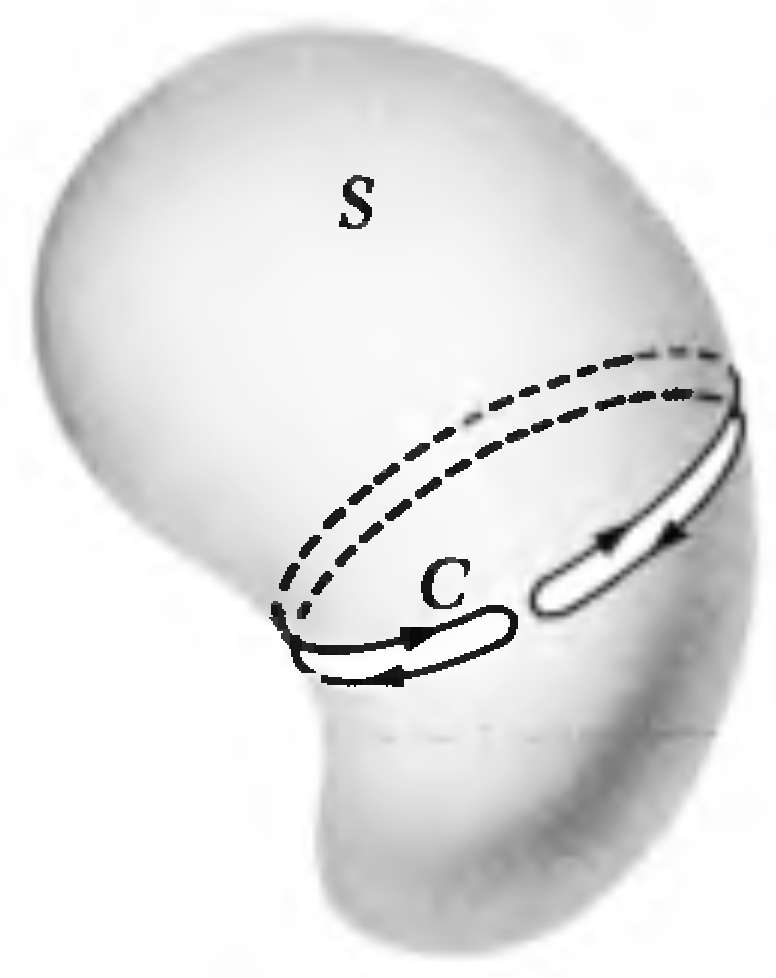
\includegraphics[width=0.33\textwidth]{ps03_02}\end{center}
  \end{enumerate}
\subsection{Solution}
  \begin{enumerate}
    \item $$\vec{\nabla}\cdot \left( \vec{\nabla} \times \vec{A} \right) = \KKdiv{\left( \frac{\partial A_z}{\partial y} - \frac{\partial A_y}{\partial z} \right)} {\left( \frac{\partial A_x}{\partial z} - \frac{\partial A_z}{\partial x} \right)} {\left( \frac{\partial A_y}{\partial x} - \frac{\partial A_x}{\partial y} \right)}{}{+}{+} = 0 $$
    \item
      \begin{figure}[ht]
        \centering
        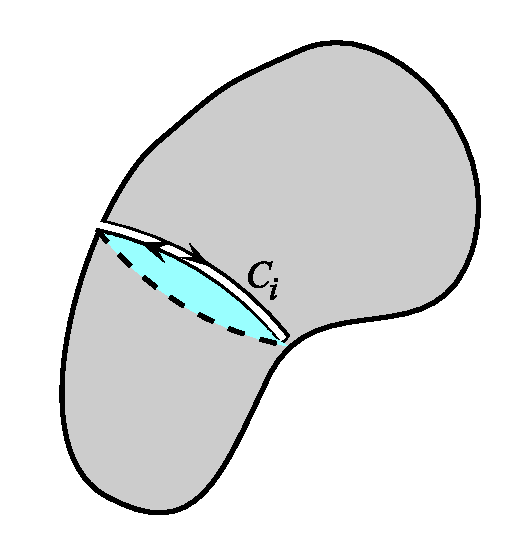
\includegraphics[width=0.33\textwidth]{ps03_sol_02}
        \caption{Balloon with a cut}
        \label{fig:balloon}
      \end{figure}
      Using Divergence theorem we get,
      $$\int \vec{\nabla}\cdot \left( \vec{\nabla} \times \vec{A} \right)\,dV = \oint \left( \vec{\nabla} \times \vec{A} \right)\cdot d\vec{S}$$
      where (for this problem) the surface area element is $d\vec{S}$ instead of the usual $d\vec{A}$ since the vector $\vec{A}$ has already been assigned a different meaning. We can evaluate the surface integral by summing up the surface integral over several infinitesimal cuts (see \autoref{fig:balloon}).
      Hence,
      $$\oint  \left( \vec{\nabla} \times \vec{A} \right)\cdot \hat{n}\,dS = \sum_i \iint_{S_i}\left( \vec{\nabla} \times \vec{A} \right)\cdot \hat{n}\,dS$$
      where $S_i$ denotes the region enclosed by $C_i$ on the curved surface (white area). Using Stoke's law we get,
      $$\sum_i \oint_{S_i}\left( \vec{\nabla} \times \vec{A} \right)\cdot \hat{n}\,dS = \sum_i \oint_{S_i} \vec{A}\cdot \vec{dr}$$
      Note that the line integral around the infinitesimal ``cut'' ($C_i$) must vanish, as it is a sum of a line integral evaluated in the clockwise direction and the same integral evaluated in the counter-clockwise direction. Hence,
      $$\sum_i \oint_{S_i} \vec{A}\cdot \vec{dr} = 0 \implies  \oint  \left( \vec{\nabla} \times \vec{A} \right)\cdot \hat{n}\,dS = 0 \implies \int \vec{\nabla}\cdot \left( \vec{\nabla} \times \vec{A} \right)\,dV = 0$$
      Since we evaluated the volume integral of $\vec{\nabla}\cdot \left( \vec{\nabla} \times \vec{A} \right)$ for any arbitrary volume, $\vec{\nabla}\cdot \left( \vec{\nabla} \times \vec{A}\right) = 0$.
  \end{enumerate}
\section{Problem \thesection: Stokes's Theorem in Action}
\subsection{Problem}
  Consider the vector field $\vec{F} = \hat{x} z^2 + \hat{y} x^2 - \hat{z} y^2$.
  \begin{enumerate}[(a)]
    \item Calculate $\oint \vec{F} \cdot d\vec{r}$ around a square path with
      corners $(x_0 \pm s/2,~~y_0 \pm s/2,~~0)$. The square has
      center $(x_0,y_0,0)$, side length $s$, and its sides are parallel to
      the $x$- and $y$-axes. The sense of rotation of the path
      is counter-clockwise as viewed from the $+z$ direction.
    \item Divide your answer to (a) by the area of the square, and take
      the limit as $s\rightarrow 0$.
    \item Calculate $\vec{\nabla}\times \vec{F}$ at the center of the square.
    \item Verify that your answer to (b) is equal to the normal component
      of $\vec{\nabla}\times\vec{F}$ evaluated at the center of the square.
  \end{enumerate}
\subsection{Solution}
  \begin{enumerate}[(a)]
    \item $$\oint \vec{F} \cdot d\vec{s} = \int_{x_0-s/2}^{x_0+s/2} F_x\left((x,y_0 -\frac{s}{2},0 \right) dx + \int_{y_0-s/2}^{y_0+s/2} F_x\left((x_0 +\frac{s}{2},y,0 \right)\,dy  $$ $$+ \int_{x_0+s/2}^{x_0-s/2} F_x\left((x,y_0 +\frac{s}{2},0 \right)\,dx +  \int_{y_0+s/2}^{y_0-s/2} F_x\left((x_0 -\frac{s}{2},y,0 \right)\,dy$$
      Hence,
      $$\oint \vec{F} \cdot d\vec{s} = s\left( x_0 + \frac{s}{2} \right)^2-s\left( x_0 - \frac{s}{2} \right)^2 = 2 s^2 x_0$$
    \item $$\lim_{s\rightarrow 0}\frac{1}{s^2}\oint \vec{F} \cdot d\vec{s} = 2 x_0$$
    \item $\vec{\nabla} \times \vec{F} (x_0,y_0,0)= -2 y_0 \hat x + 2 x_0 \hat z $
    \item The normal to the square points along the $\hat z$ direction. hence, the normal component of $\vec{\nabla} \times \vec{F} (x_0,y_0,0)$ is $2x_0$. This is the answer we got in part (b)!
  \end{enumerate}
\section{Problem \thesection: Gauss's Theorem in Action}
\subsection{Problem}
  Consider a vector field
  $\vec{F} = r\hat{r}$ (in spherical coordinates), and a closed
  surface $S$ that is a cube with one corner at the origin and the
  opposite corner at $(b,b,b)$.  Verify Gauss's theorem,
  $$\oint \vec{F}\cdot\hat{n}\,dS = \int (\vec{\nabla}\cdot\vec{F})\,dV,$$
  for this particular case by performing both the surface integral on the
  left side, and the volume integral on the right side, and showing that
  they are equal.
\subsection{Solution}
  \begin{figure}[h]
    \centering
    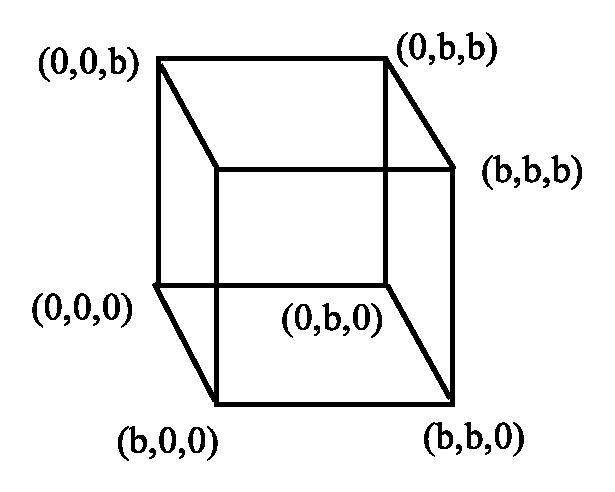
\includegraphics[width=0.5\textwidth]{ps03_sol_04}
    \caption{Cube of side $b$}
    \label{fig:cube}
  \end{figure}
  A sketch of the cube is shown in \autoref{fig:cube}. The surface integral of $\vec{F}$ over the cube is
  \begin{align*}
    \mathop{\oint}_{\text{cube}}\vec{F}\cdot\hat{n}\,dA & = -\int_{0}^b\int_{0}^b\vec{F}(0,y,z)\cdot \hat x\,dy\,dz + \int_{0}^b\int_{0}^b\vec{F}(b,y,z)\cdot \hat x\,dy\,dz \\
    & \phantom{=} -\int_{0}^b\int_{0}^b\vec{F}(x,0,z)\cdot \hat y\,dz\,dx + \int_{0}^b\int_{0}^b\vec{F}(x,b,z)\cdot \hat y\,dx\,dz \\
    & \phantom{=} -\int_{0}^b\int_{0}^b\vec{F}(x,y,0)\cdot \hat z\,dx\,dy + \int_{0}^b\int_{0}^b\vec{F}(x,y,b)\cdot \hat z\,dx\,dy \\
    & = 0 + b^3 -0 + b^3 - 0 + b^3 = 3 b^3
  \end{align*}
  Now, $\vec{\nabla}\cdot \vec{F} =3$. Hence,
  $$\int \vec{\nabla}\cdot \vec{F}\,dV = 3 \mathop{\int}_{\text{cube}}\,dV = 3 b^3$$

  Thus we have verified that,
  $$\oint \vec{F}\cdot\hat{n}\,dA = \int (\vec{\nabla}\cdot\vec{F}) dV$$
\section{Problem \thesection: Purcell 2.4 \& 2.8 --- One more time}
\subsection{Problem}
  \begin{enumerate}[(a)]
    \item Describe the charge distribution that goes with the following potential:
      \begin{align*}
        \phi & = x^2 + y^2 + z^2 & \text{for }x^2 + y^2 + z^2 < a^2 \\
        \phi & = -a^2 + \frac{2a^3}{(x^2 + y^2 + z^2)^{1/2}} & \text{for }a^2 < x^2 + y^2 + z^2
      \end{align*}
      Discuss what happens at the boundary ($x^2 + y^2 + z^2 = a^2$).
    \item Consider a very long cylinder of radius $R$ that is filled with a uniform charge density $\rho$ (Fig. 2.17).  Again, find the electric field, $\vec{E}$, both inside and outside the cylinder, by integrating Poisson's equation: $\vec{\nabla} \cdot \vec{E} = 4 \pi \rho$.

      Be sure that the $\vec E$ field inside and the $\vec E$ field outside match at the boundary (i.e., at $R$).
      \begin{center}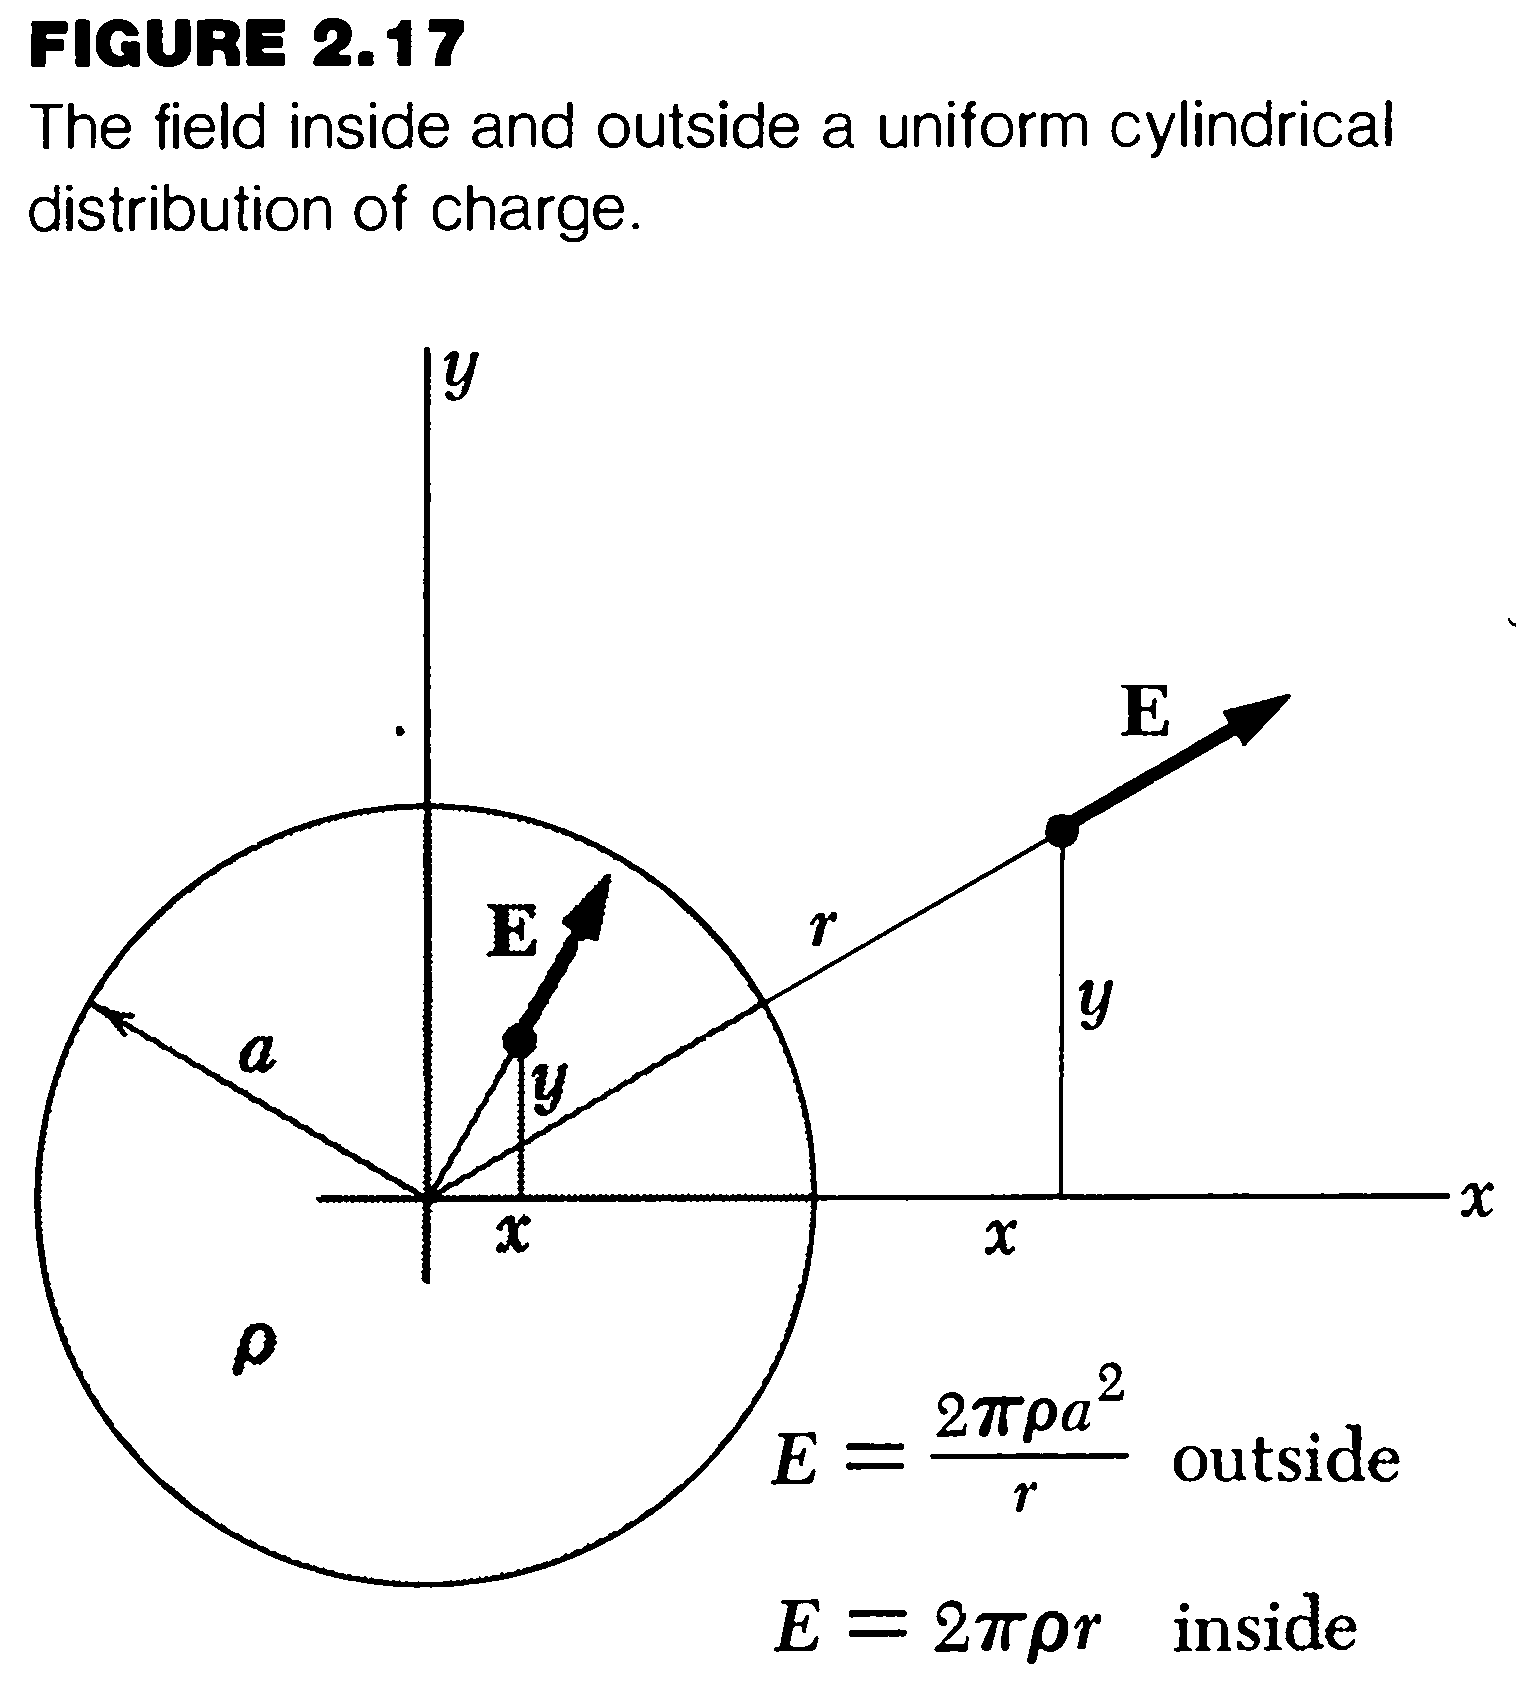
\includegraphics[width=0.5\textwidth]{ps02_2}\end{center}
  \end{enumerate}
\subsection{Solution}
  \begin{enumerate}[(a)]
    \item For $x^2+y^2+z^2<a^2$, $\phi=x^2+y^2+z^2$, recall from Problem Set 2 that
      \begin{align*}
        \vec{E} & = -\nabla\phi\\
                & = -\frac{\partial\phi}{\partial x}\hat{x}
        -\frac{\partial\phi}{\partial y}\hat{y}
        -\frac{\partial\phi}{\partial z}\hat{z}\\
                & = -2x\hat{x}-2y\hat{y}-2z\hat{z},
      \end{align*}
      or $\vec{E}=(E_x,E_y,E_z)=(-2x,-2y,-2z)$.  Then
      \begin{align*}
        \rho & = \frac{1}{4\pi}\nabla\cdot\vec{E}\\
             & = \frac{1}{4\pi}(\frac{\partial E_x}{\partial x}+
        \frac{\partial E_y}{\partial y}+\frac{\partial E_z}{\partial z})\\
             & = -\frac{3}{2\pi}.
      \end{align*}
      For $x^2+y^2+z^2>a^2$, $\phi=-a^2+\frac{2a^3}{(x^2+y^2+z^2)^{1/2}}$, recall from Problem Set 2 that
      \[\vec{E}=\left(\frac{2a^3 x}{(x^2+y^2+z^2)^{3/2}}\right)\hat{x}+
      \left(\frac{2a^3 y}{(x^2+y^2+z^2)^{3/2}}\right)\hat{y}+
      \left(\frac{2a^3 z}{(x^2+y^2+z^2)^{3/2}}\right)\hat{z}.\]
      Then
      \[\rho=0.\]
      That's not the end of the story: we should be careful of the boundary!
      Take a limit of $x^2+y^2+z^2\rightarrow a^2$ from both inside and
      outside; the fields are not the same.  This indicates there are some surface
      charge density $\sigma$ on the boundary $x^2+y^2+z^2=a^2$.

      Let
      $a^-\equiv \smashoperator{\lim\limits_{\substack{\varepsilon\rightarrow 0 \\ \varepsilon>0}}}(a-\varepsilon)$
      and $a^+\equiv \smashoperator{\lim\limits_{\substack{\varepsilon\rightarrow 0 \\ \varepsilon>0}}}(a+\varepsilon)$.
      \begin{align*}
        \vec{E_1}& = \vec{E}\left(x^2+y^2+z^2=(a^-)^2\right)=-2x\hat{x}-2y\hat{y}-2z\hat{\bf
          z}\\
        \vec{E_2}& = \vec{E}\left(x^2+y^2+z^2=(a^+)^2\right)= 2x\hat{x}+2y\hat{y}+2z\hat{\bf
          z}\\
        |\vec{E_2}-\vec{E_1}|& = |4x\hat{x}+4y\hat{y}+4z\hat{z}|\\
          & = 4\sqrt{x^2+y^2+z^2}=4a\\
        \sigma & = |\vec{E_2}-\vec{E_1}|/4\pi =+a/\pi.
      \end{align*}


    \item Outside the cylinder the differential form of Gauss's law takes the following form (in cylindrical coordinates)
      $$\frac{1}{r} \frac{\partial}{\partial r} \left( r E^{\mbox{\tiny out}}_r \right)  = 0$$
      Inside the cylinder,
      $$\frac{1}{r} \dr \left( r E^{\text{in}}_r \right)  = 4 \pi \rho$$
      Solving the above equations we find,
      $$E^{\text{out}}_r = \frac{A}{r}\mbox{ and }E^{\text{in}}_r = 2\pi \rho r + \frac{B}{r}$$
      Note that $B$ must vanish for the electric field to be well defined at the origin. Equating, the electric field inside and outside we get,
      $$E^{\text{out}}_r(R) = E^{\text{in}}_r(R) \implies A = 2\pi R^2 \rho$$
      Hence,
      $$E^{\text{out}}_r = \frac{2\pi R^2 \rho}{r} \text{ and } E^{\text{in}}_r=2\pi r \rho$$
  \end{enumerate}
\section{Problem \thesection: Potential of an Electric Dipole}
\subsection{Problem}
  Compute the potential $\varphi(x,y,z)$ of a dipole charge configuration.  The dipole consists of a charge $+q$ located at $z = a/2$ and a charge $-q$ located at $z=-a / 2$.
  \begin{enumerate}[(a)]
    \item Write down $\varphi(x,y,z)$ (i.e., in Cartesian coordinates).
    \item Expand $\varphi(x,y,z)$ in a Maclaurin series (i.e., a Taylor series about $a=0$) to first order in $a$.
    \item Convert your results to spherical coordinates: $\varphi(r, \theta, \phi)$.
    \item Compute $\vec{\nabla}\varphi(r, \theta, \phi)$, in spherical coordinates, to find $\vec{E}$. % and compare your results with what you found in Problem \#6 of pset \#1.
  \end{enumerate}
\subsection{Solution}
  \begin{enumerate}[(a)]
    \item The potential at a point $(x,y,z)$ due to the dipole is given by
      \begin{equation}
        \varphi(x,y,z) = \frac{q}{\left( x^2 + y^2 +(z-a/2)^2 \right)^{1/2}} - \frac{q}{\left( x^2 + y^2 +(z+a/2)^2 \right)^{1/2}} \label{eq:potdip}
      \end{equation}
    \item Expanding the potential in \autoref{eq:potdip} to first order in $a$ we get
      $$\varphi(x,y,z) = \frac{q}{\left( x^2 + y^2 +z^2 \right)^{1/2}}\left( \left( 1+ \frac{1}{2} \frac{az}{x^2 + y^2 + z^2} \right) - \left(1-\frac{1}{2} \frac{az}{x^2 + y^2 + z^2} \right)\right) + \mathcal O(a^2)$$
      After some simplification we get
      \begin{equation}  \varphi(x,y,z) = \frac{q az}{\left( x^2 + y^2 +z^2 \right)^{3/2}} \label{eq:potdipsim}\end{equation}
    \item The expression for the dipole potential in \autoref{eq:potdipsim} can be written in spherical polar coordinates as follows,
      $$\varphi(r,\theta,\phi) = \frac{q a \cos \theta}{r ^2}$$
    \item The electric field is given by
      \begin{align*}
        \vec{E} & = - \vec{\nabla}\varphi(r,\theta,\phi) = - \hat r \dr \left( \frac{qa \cos \theta}{r^2} \right) - \hat\theta \frac{1}{r}\dtheta \left( \frac{qa \cos \theta}{r^2} \right) \\
          & = \hat r\frac{2 qa \cos \theta}{r^3} + \hat\theta \frac{qa \sin \theta}{r^3}
      \end{align*}
      %This is same as the electric field we had found in problem \#6 of pset \#1 except for the orientation.
  \end{enumerate}
\section{Problem \thesection: Purcell 2.29}
\subsection{Problem}
  One of two nonconducting spherical shells of radius $a$ carries
  a charge $Q$ uniformly distributed over its surface, the other a charge
  $-Q$, also uniformly distributed. The spheres are brought together
  until they touch. What does the electric field look like, both outside
  and inside the shells? How much work is needed to move them far
  apart?
\subsection{Solution}
  The electric field due to a single spherical shell of radius $a$ and charge $Q$ is given by
  $$\vec{E}(r) =
    \begin{cases}
      0  & \text{for }|\vec{r} - \vec{r}_{0}|<a \\
      \frac{Q \left(\vec{r} - \vec{r}_{0}\right)}{|\vec{r} - \vec{r}_{0}|^3} & \text{for }|\vec{r} - \vec{r}_{0}|>a
    \end{cases}
  $$
  where $\vec{r}$ denotes the position vector of the point at which electric field is evaluated and $\vec r_0$ denotes the position vector of the center of the spherical shell.  In class, we usually put $\vec r_0 = \vec 0$.

  We will now evaluate the electric field due to two non-conducting spherical shells touching each other. Without loss of generality, we can assume that the centers are located at $(0,0,\pm a)$.
  \begin{center}
    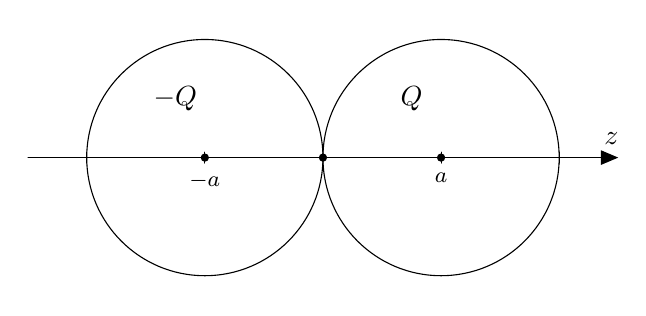
\begin{tikzpicture}[line cap=round,line join=round,>=triangle 45,x=1.5cm,y=1.5cm]
      \clip(-2.5,-1.1) rectangle (2.5,1.1);
      \draw[->,color=black] (-10,0) -- (2.5,0);
      \foreach \x in {-2,-1,1,2}
        \draw[shift={(\x,0)},color=black] (0pt,2pt) -- (0pt,-2pt) node[below] {\footnotesize\ifnum\x=-1$-a$\fi\ifnum\x=1$a$\fi};
      \draw[color=black] (2.3,0.03) node [anchor=south west] {$z$};
      %\draw[color=black] (0pt,-20pt) node[center] {\footnotesize $0$};
      \draw(1,0) circle (1);
      \draw(-1,0) circle (1);
      \fill [color=black] (-1,0) circle (1.5pt);
      \fill [color=black] (1,0) circle (1.5pt);
      \fill [color=black] (0,0) circle (1.5pt);
      \draw[color=black] (0.75,0.5) node {$Q$};
      \draw[color=black] (-1.25,0.5) node {$-Q$};
    \end{tikzpicture}
  \end{center}
  The electric field is given by the superposition of the electric field of each spherical shell. Hence,
  $$\vec E(\vec{r}) =
    \begin{cases}
      -\frac{Q \left(\vec{r}  + a \hat z \right)}{|\vec{r} + a \hat z|^3} & \text{for }|\vec{r} - a \hat z| < a \\
      \frac{Q \left(\vec{r}  - a \hat z \right)}{|\vec{r} - a \hat z|^3} & \text{for }|\vec{r} + a \hat z| < a \\
      \frac{Q \left(\vec{r}  - a \hat z \right)}{|\vec{r} - a \hat z|^3} - \frac{Q \left(\vec{r}  + a \hat z \right)}{|\vec{r} + a \hat z|^3} & \text{otherwise}
    \end{cases}
  $$

  \begin{figure}[ht]
    \centering
    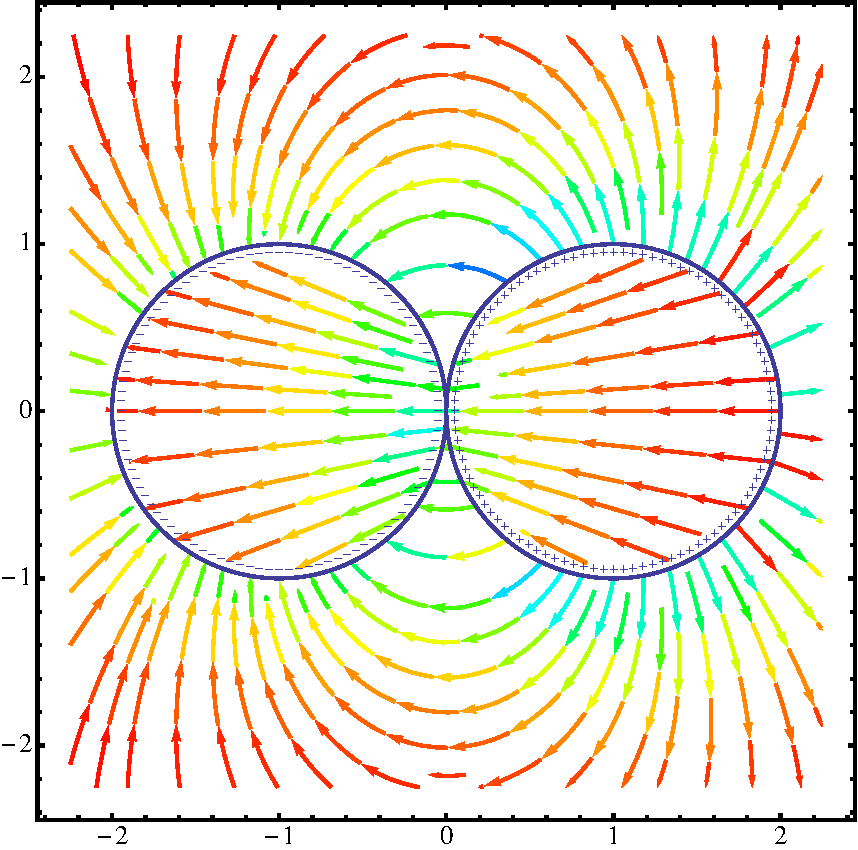
\includegraphics[width=0.33\textwidth]{ps03_sol_07}
    \caption{Electric Field Lines}
    \label{fig:TwoSpheres}
  \end{figure}

  \autoref{fig:TwoSpheres} shows a sketch of the electric field lines. Note that $\vec{E}$ depends on $r$ and $\theta$ but not $\phi$.\footnote{$|r\pm a \hat z| = \left(r^2 + a^2 \pm 2 ra\cos \theta \right)^{1/2}$}

  We will treat the spherical shells as point charges to calculate the work done to move these shells far apart. This is justified because the average potential of one sphere in presence of the other is the potential at its center.  %We will prove this result in Problem 9.
  Hence, the work done to move these two shells far apart is
  $$W = \frac{Q^2}{2a}.$$
\section{Problem \thesection: Purcell 2.14 (Laplace's equation)}
\subsection{Problem}
  Does the function $f(x, y) = x^2 + y^2$ satisfy the two-dimensional
  Laplace equation? Does the function $g(x, y) = x^2 - y^2$?
  Sketch the latter function, calculate the gradient at the points $(x = 0, y = 1)$;
  $(x = 1, y = 0)$; $(x = 0, y = -1)$; and $(x = -1, y = 0)$ and indicate
  by little arrows how these gradient vectors point.
\subsection{Solution}
  Since $\nabla^2 f(x,y)=\frac{\partial^2 f}{\partial x^2}+\frac{\partial^2 f}{\partial y^2}=2+2=4$, $f(x,y)$ does not satisfy the 2-D Laplace equation.

  However, $g(x,y)$ does, since $\nabla^2 g(x,y)=\frac{\partial^2 g}{\partial x^2}+\frac{\partial^2 g}{\partial y^2}=2-2=0$.

  $$\nabla g(x,y)=\frac{\partial g}{\partial x} \hat{x} + \frac{\partial g}{\partial y} \hat{y}=2x\hat{x}-2y\hat{y}.$$
  \begin{align*}
    \nabla g|_{(0,1)} & = -2\hat{y}, & \nabla g|_{(1,0)} & = 2\hat{x}, \\
    \nabla g|_{(0,-1)} & = 2\hat{y}, & \nabla g|_{(-1,0)} & = -2\hat{x}.
  \end{align*}

  \begin{figure}[ht]
    \centering
    \subfloat[]{\label{fig:line_saddle}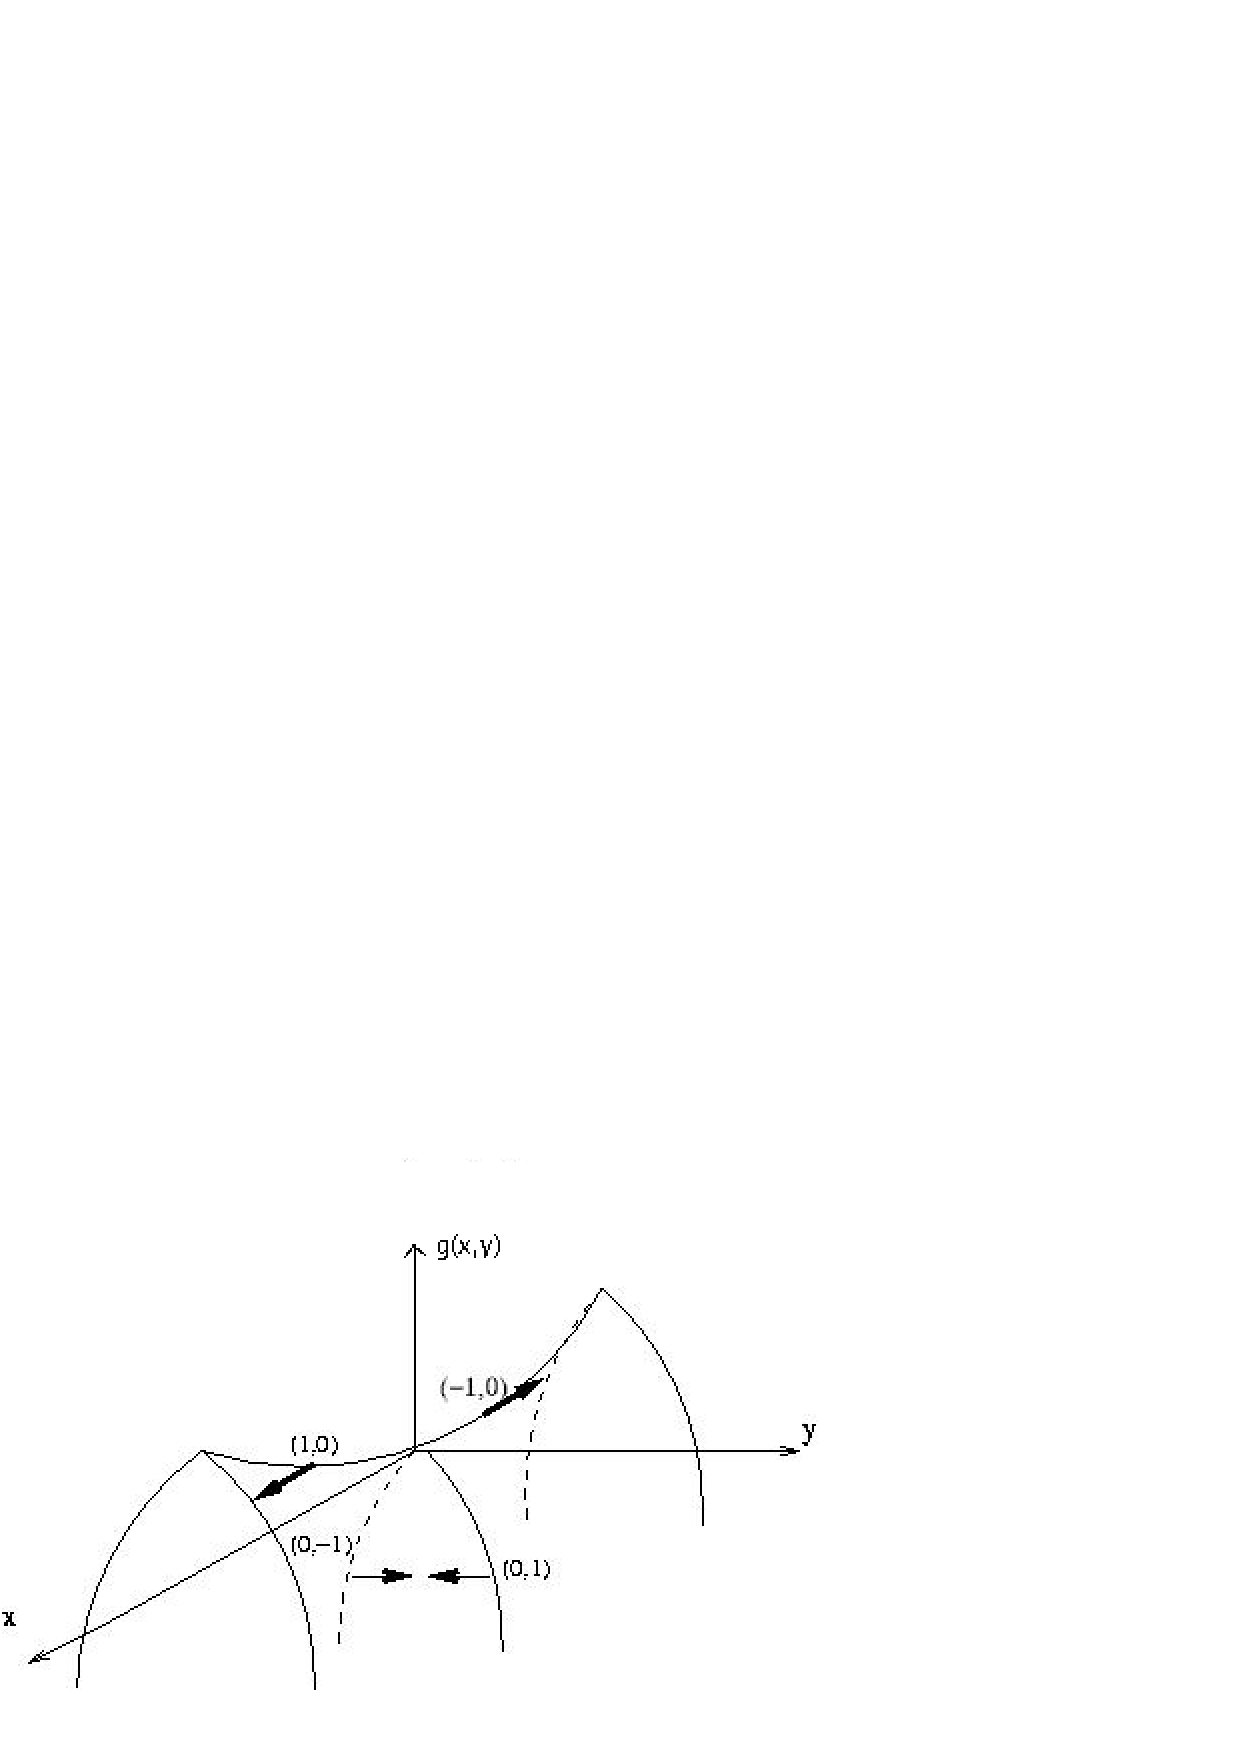
\includegraphics[width=4in]{ps03_sol_08_a}}
    \subfloat[]{\label{fig:mesh_saddle}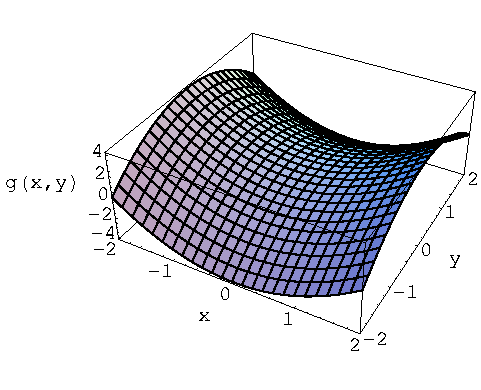
\includegraphics[width=2.5in]{ps03_sol_08_b}}
    \caption{saddle shape}
    \label{fig:saddle}
  \end{figure}

  \noindent\textsc{Note}: $\nabla g|_{(x=0,y=1)}$ anti-parallel to $y$-axis, $\nabla
  g|_{(x=1,y=0)}$ parallel to $x$-axis, $\nabla g|_{(x=0,y=-1)}$ parallel
  to $y$-axis,$\nabla g|_{(x=-1,y=0)}$ anti-parallel to $x$-axis.  The
  gradient vectors are all in $xy$-plane.
\section{Problem \thesection: Electric field, potential, and flux}
\subsection{Problem}
  A hollow spherical shell carries charge density $\rho = k/r^2$ in the
  region $a \le r \le b$:
  \begin{center}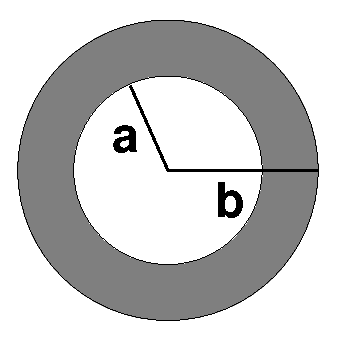
\includegraphics[width=3.5cm]{ps03_09}\end{center}
  \begin{enumerate}[(a)]
    \item Find the electric field $\vec E$ everywhere in space
    \item Find the potential $\phi$ everywhere in space.
    \item Calculate the electric flux through
      \begin{enumerate}[(i)]
        \item A concentric sphere with radius $r_1 > b$
        \item A concentric sphere with radius $a \le r_2 \le b$
        \item A concentric sphere with radius $r_3 < a$
        \item A nonconcentric sphere centered on \emph{any} point on the
          outer surface of the shell, and of radius $r_4 = 2b$.
      \end{enumerate}
  \end{enumerate}
\subsection{Solution}
  \begin{enumerate}[(a)]
    \item From Gauss's Law:
      \begin{align*}
        r<a,   & \vec{E}=0\\
        a<r<b, & 4\pi r^2 E = 4\pi Q_{\text{enclosed}} = 4\pi\int_a^r \frac{k}{r^2}4\pi r^2\,dr=(4\pi)^2k(r-a)\\
               & \Rightarrow E = 4\pi \frac{k(r-a)}{r^2}\\
        r>b,   & 4\pi r^2 E = 4\pi Q_{\text{enclosed}} = 4\pi\int_a^b \frac{k}{r^2}4\pi r^2\,dr=(4\pi)^2k(b-a)\\
               & \Rightarrow E= 4\pi \frac{k(b-a)}{r^2}
      \end{align*}

    \item Assume $\phi(r\rightarrow\infty)=0$
      \begin{align*}
        r>b,  &  \phi(r)-\phi(\infty)=-\int_\infty^r \vec{E}(r') \cdot d\vec{r'} \\
              & \Rightarrow \phi(r)=-\int_\infty^r 4\pi \frac{k(b-a)}{r'^2}dr'=4\pi \frac{k(b-a)}{r}.\\
        a<r<b,& \phi(r)-\phi(b)=-\int_b^r\vec{E}(r') \cdot d\vec{r'},\\
              & \Rightarrow \phi(r)= \phi(b)-\int_b^r\vec{E}(r') \cdot d\vec{r'}=4\pi k [1-a/r-\ln (r/b)].\\
        r<a,  & \phi(r)= 4\pi k\ln (\frac{b}{a}).
      \end{align*}

    \item Flux
      \begin{enumerate}[(i)]
        \item For concentric sphere with $r_1>b$, flux $\phi_1=(4\pi)^2k(b-a)$.\\
        \item For $a<r_2<b$ flux $\phi_2=(4\pi)^2k(r_2-a)$.\\
        \item For $r<a$ flux $\phi_3$ is zero since the electric field is zero.\\
        \item From Gauss's law, flux $\phi_4=\oint\vec{E} \cdot\,ds = 4\pi
          Q_{\text{total}} = (4\pi)^2 k(b-a)$
      \end{enumerate}
  \end{enumerate}
\section{Problem \thesection: Purcell 2.20 (Potential at the center of a gold nucleus)}
\subsection{Problem}
  As a distribution of electric charge, the gold nucleus can be
  described as a sphere of radius \SI{6e-13}{\centi\meter} with a charge $Q = 79e$
  distributed fairly uniformly through its interior. What is the potential
  $\phi_0$ at the center of the nucleus, expressed in megavolts? (First derive
  a general formula for $\phi_0$ for a sphere of charge $Q$ and radius $a$. Do
  this by using Gauss's law to find the internal and external electric field
  and then integrating to find the potential.)
  \begin{flushright} \emph{Ans}. $\phi_0 = 3Q/2a = \num{95000}\text{ statvolts} = 28.5\text{ megavolts}$. \end{flushright}
\subsection{Solution}
  For a uniformly charged sphere of radius $a$,
  \[ \vec{E} = \begin{cases} \frac{Q}{r^2}\hat{r} & r>a \\ \frac{Qr}{a^3}\hat r & r\le a \end{cases} \]
  Since the potential is zero at infinity, the potential at any point $P$ is
  \[ \phi(P) = -\int_\infty^P \vec{E}\cdot d\vec s. \]
  We can make the path of integration come radial straight in. If the point $P$ has $r<a$,
  \[ \phi(r) = -\int_\infty^r E_{r'}\,dr' = -\int_\infty^a \frac{Q}{r'^2}\,dr' - \int_a^r\frac{Qr'}{a^2}\,dr' = \frac{Q}{a} - \frac{Qr^2}{2a^3} + \frac{Q}{2a} \]
  In SI units,
  \[ \phi(0) = \frac{1}{4\pi\epsilon_0}\frac{3Q}{2a} = \frac{3\cdot79(\SI{1.6e-19}{\coulomb})}{4\pi(\SI{8.85e-12}{\coulomb\squared\per\newton\per\meter\squared})2(\SI{6e-15}{\meter})} = \SI{28.4}{\mega\volt}. \]
\end{document}
